\documentclass[]{article}

\usepackage{hyperref}
\usepackage{microtype}
\usepackage{float}
\usepackage{graphicx}

\title{\texttt{23\_14} Web Scraper}
\author{boa (\texttt{boaboa})}

\begin{document}

\maketitle

\begin{abstract}

%Write a program that extracts and aggregates news headlines from various sources.
%With Copilot, you can get help on understanding various web scraping techniques and libraries.



\end{abstract}

\pagebreak

\section{Tervezés}

A ChatGPT promptolásánál mindig angol nyelvű szöveget használtam, mert abban jobb a modell (lévén, hogy tanítás abból közben többet látott).

\begin{figure}[H]
	\centering
	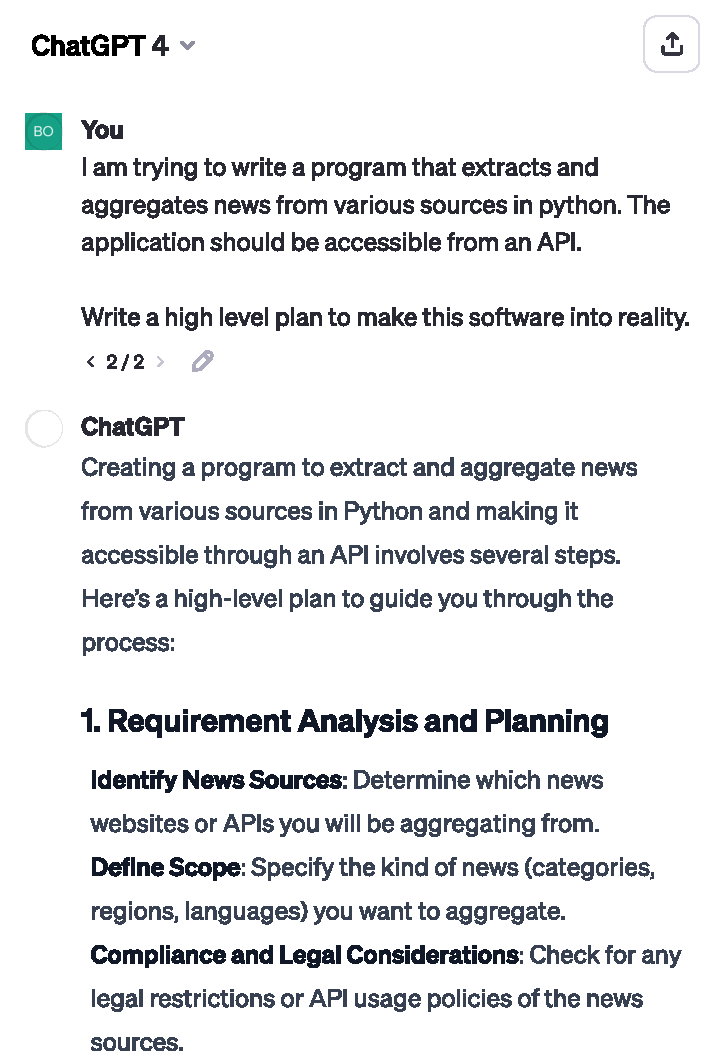
\includegraphics[width=0.7\textwidth]{prompt_1.pdf}
	\caption{Kezdeti prompt (nem teljes válasz)}
\end{figure}

A ChatGPT kimenetét megvizsgálva és saját tudásomra támaszkodva úgy döntöttem RSS folyamok periódikus letöltésével fogom az új híreket megszerezni. A teljes szöveghez viszont általában csak az cikket tartalmazó oldal letoltése és értelmezése után lehet hozzáférni, erre Beautiiful Soup Python könyvtárat választottam. Az adatok eltárolását az egyszerűség kedvéért egy lokális Sqlite adatbázissal oldottam meg. Végül pedig az adatokat FastApi python könyvtár segítségével tettem elérhetővé egy API endpointon.

\section{Megoldás}

\section{Verziókövetés}

A megoldás és a dokumentáció forráskódja a következő git repository-ban elérhető: \url{https://github.com/boapps/hu-news-scraper}



\end{document}
